\documentclass{article}
\usepackage[table]{xcolor}

\usepackage[utf8]{inputenc}
\usepackage{graphicx}
\usepackage{caption}
\usepackage{float}
\usepackage{verbatim}
\usepackage{amsmath}
% \usepackage{jmath}
% \usepackage{multirow}
\usepackage[margin=1.2in]{geometry}
\usepackage{fancyhdr}
\usepackage{bm}
% \usepackage{makecell}
\usepackage{mathrsfs}
% \usepackage{minted}

\makeatletter
\renewcommand*\env@matrix[1][*\c@MaxMatrixCols c]{%
  \hskip -\arraycolsep
  \let\@ifnextchar\new@ifnextchar
  \array{#1}}
\makeatother
\newcommand\numberthis{\addtocounter{equation}{1}\tag{\theequation}}

\usepackage{graphicx}
\usepackage{array}
\usepackage{listings}
% \usepackage[export]{adjustbox}
% \usepackage{minted}

\usepackage[colorlinks=true, allcolors=blue]{hyperref}

\pagestyle{fancy}

\title{{\Huge \bfseries Lavax manual}}
\author{Daniel Karlsson (danielk5@kth.se)}
\date{June 26, 2019}

\begin{document}

\maketitle

\tableofcontents

% \begin{abstract}

% \end{abstract}

\section{Introduction}
Lavax (LAMMPS VASP Exchanger) is a program for optimizing VASP MD\footnote{Molecular Dynamcics} simulations when some atoms in the simulation cell may experience strong local compression conditions. This may be the case when studying ballistic collisions of atoms as a result from interaction with high energy radition. Lavax uses the program LAMMPS\footnote{Large-scale Atomic/Molecular Massively Parallel Simulator}, which uses methods based on classical mechanics, to predict the trajectories of the atoms in the simulation cell to check if any will come in close proximity with each other. If so, lavax will select a more accurate hard potential (which includes semi-core electrons) for those atoms before running the simulation for a few ionic steps in VASP, illustrated in Fig.~\ref{fig:pred}.
% The rest of the atoms will use a soft potential with a minimal set of valence electrons.
The whole process is repeated for a number of iterations (set by the parameter \texttt{LAVAX\_ITERATIONS} in lavax.conf) of prediction and simulation.
% \newline \\
% Lavax first uses LAMMPS to predict the trajectories for some short time period and checks which atoms will experience strong local compression. These atoms are then selec
\begin{figure}[H]
  \centering
  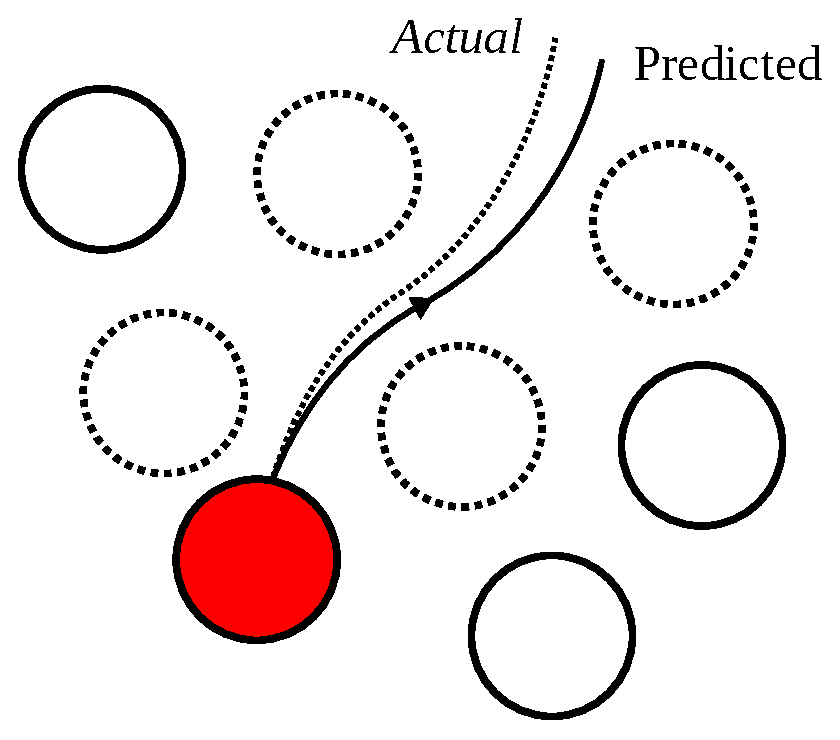
\includegraphics[scale=0.5]{img/pred.eps}
  \caption{The predicted path in LAMMPS an atom may take v.s. the actual path it will take in VASP. The dashed atoms are those whose distance is short enough to warrant a more accurate potential during a run in VASP.}
  \label{fig:pred}
\end{figure}

\subsection{Dependencies}
Lavax requires
\begin{itemize}
\item Boost C++ library (\url{https://www.boost.org/}). Recommended version $\ge$ 1.58.0.
\item C++14 compliant compiler. Recommended: g++, version $\ge$ 5.
\item GNU Build System.
\item LAMMPS, compiled using the MANYBODY and USER-MEAMC packages\footnote{\url{https://lammps.sandia.gov/doc/Packages_details.html}}.
\item VASP, (tested with version 5.4.4).
\end{itemize}

\subsection{Compilation and installation}
To compile lavax, first generate the configure script:
\begin{verbatim}
   autoreconf -i 
\end{verbatim}
Configure the environment and generate makefiles:
\begin{verbatim}
   ./configure --prefix=/desired/install/directory
\end{verbatim}
where \texttt{/desired/install/directory} is replaced by the location you want to install lavax if you don't like the default location.
\newline \\
Then build lavax with
\begin{verbatim}
   make
\end{verbatim}
and install using
\begin{verbatim}
   make install
\end{verbatim}
If boost is installed in a non-standard directory or is not included in the search path you can set this manually with either
\begin{verbatim}
   make CXXFLAGS='-I/cfs/klemming/scratch/d/danielk5/local/include
                  -L/cfs/klemming/scratch/d/danielk5/local/lib'
\end{verbatim}
or by setting the following shell variables
\begin{verbatim}
   export CPATH=$CPATH:/cfs/klemming/scratch/d/danielk5/local/include
   export LD_LIBRARY_PATH=$LD_LIBRARY_PATH:/cfs/klemming/scratch/d/danielk5/local/lib
   export LIBRARY_PATH=$LIBRARY_PATH:/cfs/klemming/scratch/d/danielk5/local/lib
\end{verbatim}

\subsubsection{Manual static build}
On some systems it might be necessary to switch between different compilers and build environments, in which case lavax may fail to run. In this case compilation can be done manually to statically link the stdc++ library and boost system/filesystem library:
\begin{verbatim}
   g++ src/main_lavax.cpp src/lavax.cpp src/init_check.cpp -std=c++14 -fpermissive
       -static-libstdc++ -static-libgcc
       -DDATADIR=\"/desired/install/directory/share/lavax\"
       -I/marconi/home/userexternal/danielk5/local/include
       -L/marconi/home/userexternal/danielk5/local/lib
       -lpthread -Wl,-Bstatic -lboost_system -lboost_filesystem -Wl,-Bdynamic -o lavax
\end{verbatim}
The executable then have to copied manually to the desired install directory.      

\section{Running Lavax}
Before running lavax, the user should create a directory to run lavax in, containing minimaly the files
\begin{itemize}
\item lavax.conf - Configuration options for lavax, see Sec.~\ref{sec:lavax_conf}.
\item predictor.in - Input file for LAMMPS for predicting the atom trajectories. A default is generated if no such file is found. It usually need to be modified to contain the correct potential file name (\texttt{LAMMPS\_POTENTIAL\_FILE} in lavax.conf) and pair style.
\item LAMMPS potential file for the desired element or alloy, e.g. W\_BN.eam.fs.
\item INCAR - Configured for MD runs.
\item POTCAR\#\_\{hard,soft\} - hard/soft VASP potential files for each element, as specified in lavax.conf.
\item Initial POSCAR as specified in lavax.conf.
\item KPOINTS
\end{itemize}

\newpage
\subsection{lavax.conf}
\label{sec:lavax_conf}
Lavax must be configured according to the following file which must be placed in the directory where lavax is run:
\begin{verbatim}
VASP_COMMAND    = mpirun -np 32 vasp533_mpi
LAMMPS_COMMAND  = lmp_serial
INIT_POSCAR     = POSCAR_init
LAVAX_ITERATIONS = 70
LAMMPS_POTENTIAL_FILE = W_BN.eam.fs
LAMMPS_PAIR_STYLE     = eam/fs

LAMMPS_HIDE_OUTPUT = false
VASP_HIDE_OUTPUT   = false

POTENTIAL_DEPARTURE_DISTANCE = 2.0

# Options for adaptive timestep in VASP and LAMMPS:
USE_ADAPTIVE_POTIM = true
MAX_DISTANCE = 0.1 # Angstroms
MAX_POTIM    = 3   # Femtoseconds

MAX_POTENTIAL_SUBSTITUTIONS = 7
MAX_VASP_NSW = 20

# List all the atomic elements in the simulation cell:
ATOMIC_SYMBOL_0 = W
VASP_POTENTIAL_FILE_HARD_0   = POTCAR0_hard
VASP_POTENTIAL_FILE_SOFT_0   = POTCAR0_soft
VASP_POTENTIAL_SYMBOL_HARD_0 = Ws
VASP_POTENTIAL_SYMBOL_SOFT_0 = W
LAMMPS_ATOMIC_SYMBOL_0       = W
\end{verbatim}
The possible flags in lavax.conf are described in Table~\ref{tab:1}.

\rowcolors{2}{gray!25}{white}
\begin{table}[H]
\centering
\caption{Description of flags in lavax.conf.\label{tab:1}}
\begin{tabular}{lp{10cm}}
  % \rowcolor{gray!50}
  \rowcolor{gray!25}
  % & Jacobi & GS & SOR \\
  \hline
  \texttt{VASP\_COMMAND} & Command used to execute VASP. \\
  \texttt{LAMMPS\_COMMAND} & Command used to execute LAMMPS. \\
  \texttt{INIT\_POSCAR} & POSCAR formatted file containing the initial state of the simulation cell. \\
  \texttt{LAVAX\_ITERATIONS} & Number of iterations Lavax will run. VASP will restart at each iteration. The total number of ionic steps will be \texttt{LAVAX\_ITERATIONS} $\cdot$ \texttt{MAX\_VASP\_NSW}. \\
  \texttt{POTENTIAL\_DEPARTURE\_DISTANCE} & The distance by which pairs atoms are in proximity with each other (when the hard and soft potential start to deviate from each other), and their potential in VASP will be set to hard. \\
  \texttt{USE\_ADAPTIVE\_POTIM} & See Section \ref{sec:adaptive_timestep}. If \texttt{false} then \texttt{POTIM} in the \texttt{INCAR} file will be used.\\
  \texttt{MAX\_VASP\_NSW} & Number of ionic steps during one lavax iteration. Since the predicted paths diverges from the actual paths in VASP, it is important not to set this too large. \\
  \texttt{MAX\_POTENTIAL\_SUBSTITUTIONS} & If the number of atoms in close proximity change by this many or more between two lavax iterations, lavax switches to hard potential on all atoms in the simulation cell and deletes the WAVECAR to avoid divergence (i.e. VASP crash). \\
  \texttt{VASP\_POTENTIAL\_FILE\_*\_\#} & POTCAR file for the hard/soft potential for element \#. These will be concatenated in proper order to POTCAR by lavax.\\
  \texttt{VASP\_POTENTIAL\_SYMBOL\_*\_\#} & The symbols for the atomic elements should not be more than two characters long due to a bug in VASP, and must be different for the hard and soft potential for the same element. \\
  \texttt{LAMMPS\_ATOMIC\_SYMBOL\_\#} & Usually the same as \texttt{ATOMIC\_SYMBOL\_\#}, the element symbol.\\
  \hline
\end{tabular}
\end{table}

\subsection{Adaptive timestep}
\label{sec:adaptive_timestep}
In the beginning of the simulation it can be of interest to take smaller time steps since a few of the atoms will have comparably high speeds (such as the PKA). Later in the simulation, the kinetic energy will distribute itself over the entire crystal and the maximum speed among all atoms will be much smaller.
A larger timestep will then suffice. We can use an adaptive time step $\Delta t$ chosen with the following condition in the beginning of each Lavax iteration:
\begin{equation*}
  \Delta t = \min{(\texttt{MAX\_DISTANCE}/v_{\text{max}},\; \texttt{MAX\_TIMESTEP})},
\end{equation*}
where $v_{\text{max}}$ is the maximum speed among all atoms in the crystal, \texttt{MAX\_DISTANCE} is the maximum tolerated distance any atom may travel during one ionic step and \texttt{MAX\_TIMESTEP} is the maximum tolerated time step so that we don't select an unfeasibly large time step.

\subsection{\texttt{INIT\_POSCAR}}
The initial POSCAR must contain a line with the potential symbols, as specified in the lavax.conf file.
\begin{verbatim}
BCC Xx 
1.0
6.36000000 0.00000000 0.00000000
0.00000000 6.36000000 0.00000000
0.00000000 0.00000000 6.36000000
W Ws                              <- This line must not be omitted!
14 2
Cartesian
0.00000000 0.00000000 0.00000000
1.59000000 1.59000000 1.59000000
...
\end{verbatim}

\textit{Note: } The symbols for the atomic elements (\texttt{VASP\_POTENTIAL\_SYMBOL\_*}) should not be more than two characters long due to a bug in VASP.

\newpage
\section{Determining \texttt{POTENTIAL\_DEPARTURE\_DISTANCE}}
VASP provides a large number of PAW\footnote{Projector Augmented Wave} potentials. For some elements, several PAW versions exist, where the standard version generally has no name extension. The extensions \texttt{\_pv} and \texttt{\_sv} imply that the $p$ and $s$ semi-core states are treated as valence states (i.e. for \texttt{V\_pv} the $3p$ states are treated as valence states, and for \texttt{V\_sv} the $3s$ and $3p$ states are treated as valence states). In areas far away from the core, most of the physical properties are best described by the valence electrons and the wavefunction in th core can be considered frozen, illustrated in Fig.~\ref{fig:pseudo-pot-far}. When atoms experience strong local compression it is necessary to include further (non-frozen) shells to get realistic behavior, see Fig.~\ref{fig:pseudo-pot-near}.

% To speed up convergence, a smaller basis set is used to fit the wave function in the valence region and is (unrealistically) softened in the core region, as illustrated in Fig.~\ref{fig:Sketch_Pseudopotentials}.

%The choice of cutoff radius r c is a trade-off between fast convergence and precision in the core.

% \begin{figure}[H]
%   \centering
%   \includegraphics[scale=0.6]{img/Sketch_Pseudopotentials.png}
%   \caption{When the atoms are far enough apart, it is sufficient to only include the valence electrons in the potential and the core is softened.\cite{Pseudopot}}
%   \label{fig:Sketch_Pseudopotentials}
% \end{figure}
\begin{figure}[H]
  \centering
  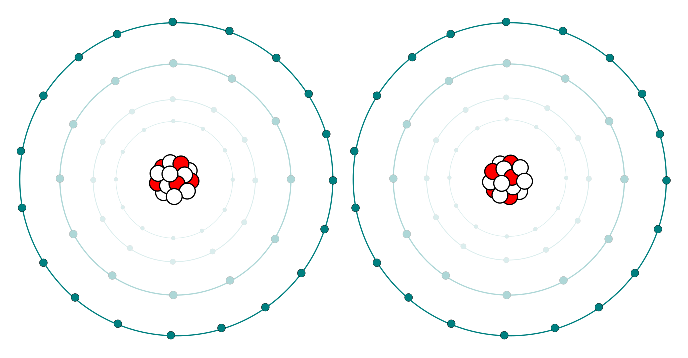
\includegraphics[scale=0.9]{img/pseudo-pot-far.eps}
  \caption{When the atoms are far enough apart, it is sufficient to only include the valence electrons in the potential.}
  \label{fig:pseudo-pot-far}
\end{figure}

\begin{figure}[H]
  \centering
  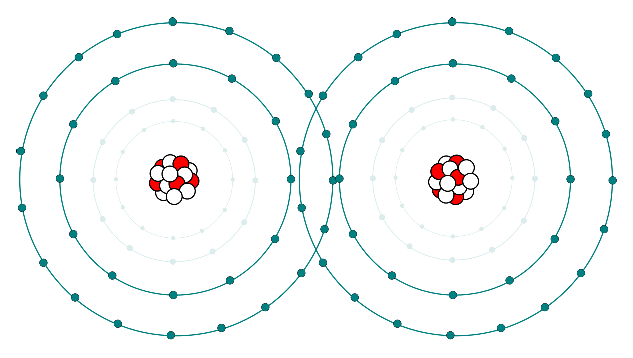
\includegraphics[scale=0.9]{img/pseudo-pot-near.eps}
  \caption{When the atoms are close enough so that their electron shells begin to overlap, it is necessary to include further shells in the potential.}
  \label{fig:pseudo-pot-near}
\end{figure}

\subsection{Methods of comparing potentials}
Only VASP is needed for this. There are two possible methods determine when two potentials (i.e. \texttt{W} and \texttt{W\_pv}) start to diverge. For both methods, the \texttt{NSW} flag in VASP is set to 0 so that the energy of the system is calculated statically. The first is a quasi-static movement of an atom as illustrated in Fig.~\ref{fig:quasi-stat-pot}. The rest of the atoms are kept at their respective lattice positions. 

\begin{figure}[H]
  \centering
  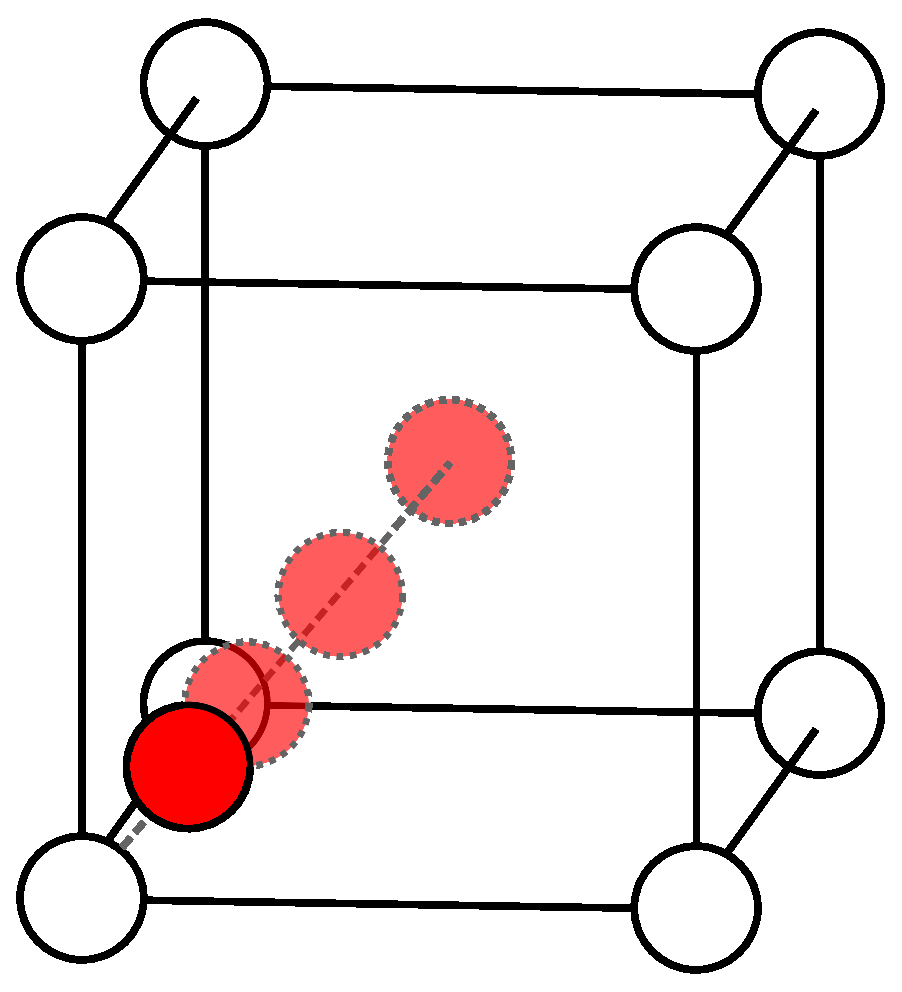
\includegraphics[scale=0.5]{img/quasi-stat-pot2.eps}
  \caption{Determining the potential energy by a quasi-static method. One of the atoms is moved closer to another atom in each iteration and the energy of the system is computed.}
  \label{fig:quasi-stat-pot}
\end{figure}

The second method is compressing the entire lattice by varying the lattice constant as illustrated in Fig.~\ref{fig:compr-pot}. This will give us a zero-level if the lattice constant $a \rightarrow \infty$.

\begin{figure}[H]
  \centering
  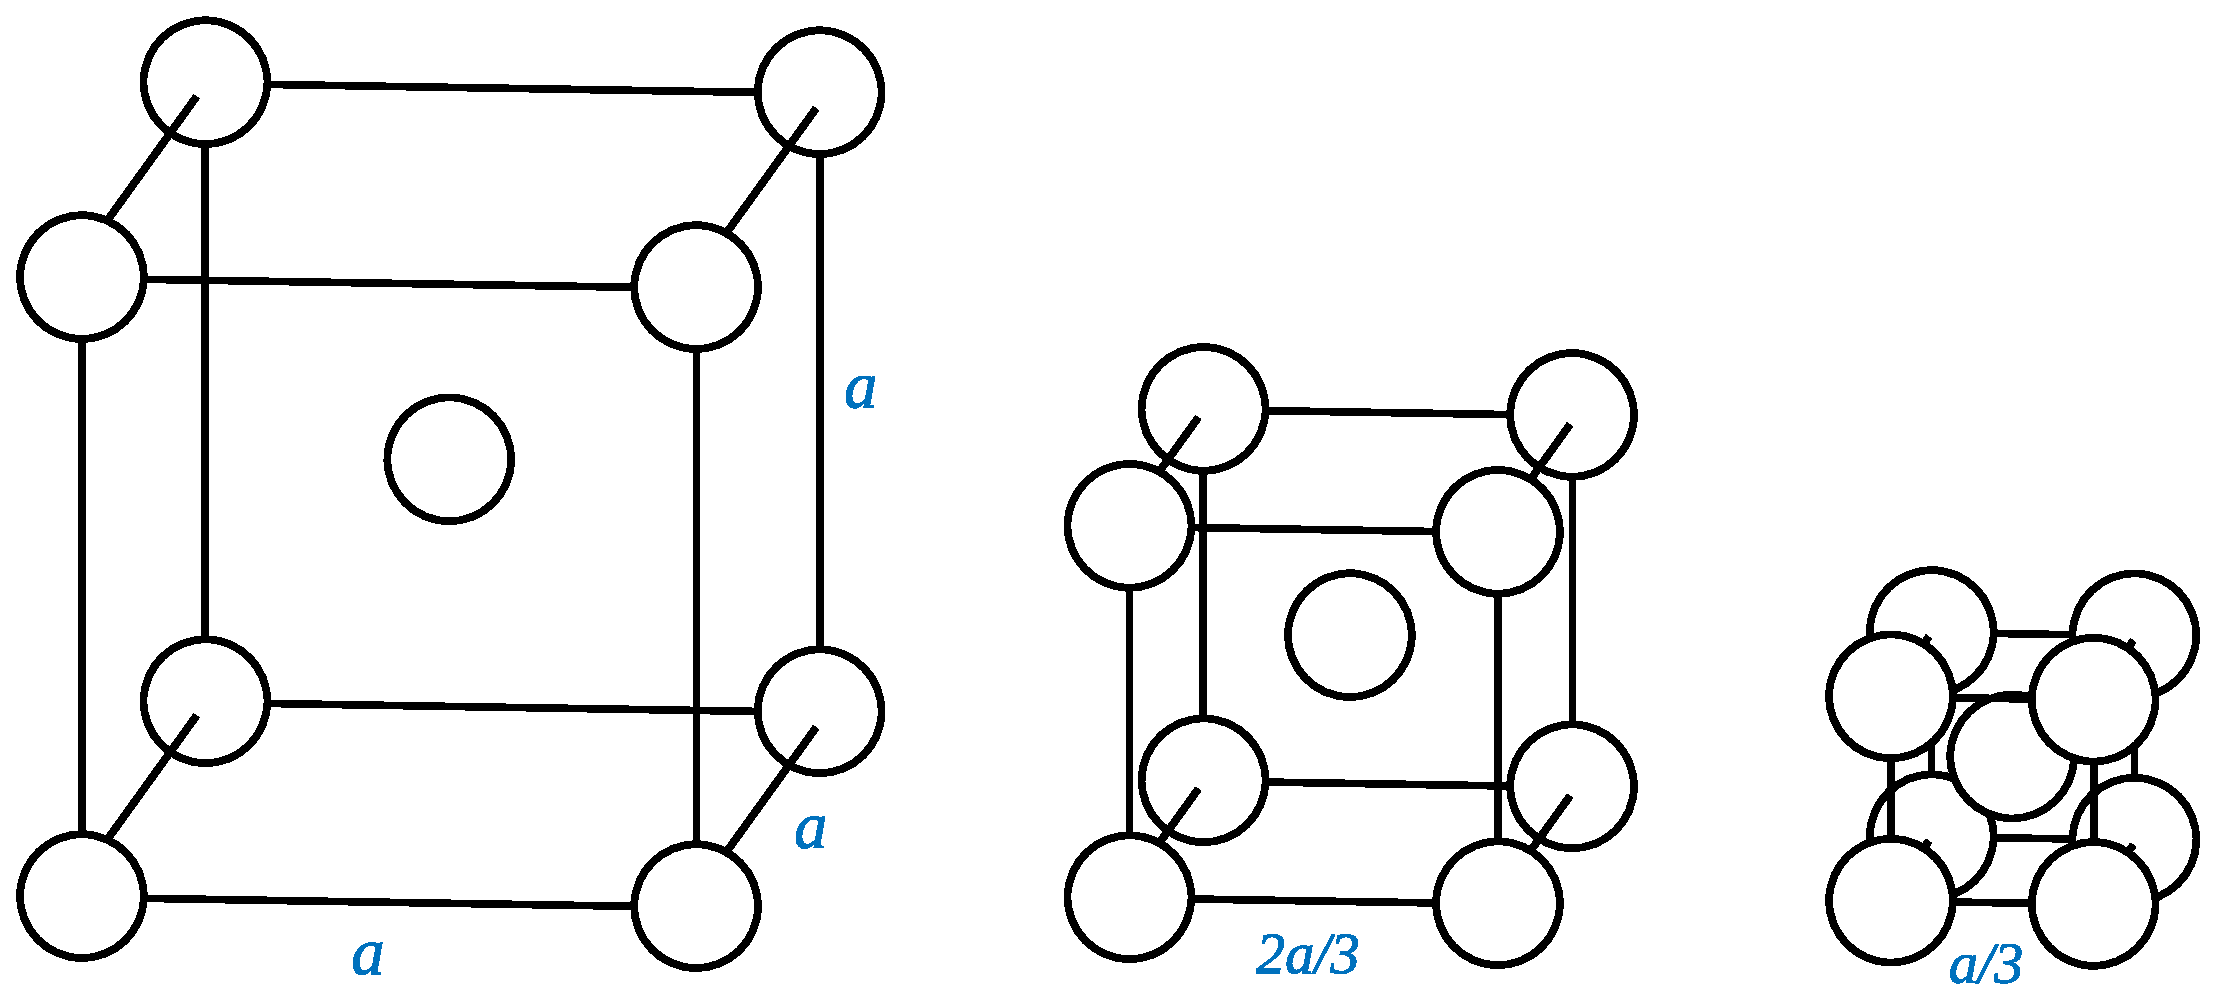
\includegraphics[scale=0.4]{img/compr-pot3.eps}
  \caption{Determining the potential energy by varying the lattice constant. This can be thought of as compressing the entire crystal.}
  \label{fig:compr-pot}
\end{figure}

Using the first method, of quasi-static movement of one atom, the potentials \texttt{W}, \texttt{W\_pv}, and \texttt{W\_sv} as a function of distance is shown in Fig.~\ref{fig:quasi-comp}, where divergence of the two can clearly be seenat short distances.

\begin{figure}[H]
  \centering
  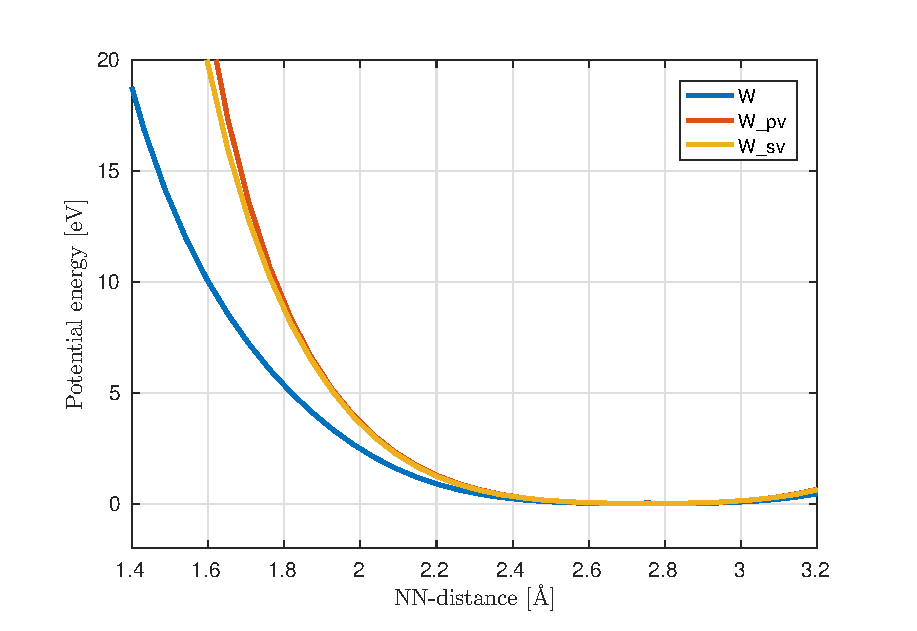
\includegraphics[scale=0.82]{img/pot-comp-quasi2.eps}
  \caption{Comparing the potential energy using the quasi-static method.}
  \label{fig:quasi-comp}
\end{figure}

Using the second method, of varying the lattice constant, we get the results in Fig.~\ref{fig:compr-comp}. Here the theoretical screened Coulumbic potential (ZBL) is inserted for comparison. From both Fig.~\ref{fig:quasi-comp} and~\ref{fig:compr-comp} we can clearly see that the potential \texttt{W} starts to become inadequate around the NN-distance $\approx 2.4$ Å, which may be chosen as \texttt{POTENTIAL\_DEPARTURE\_DISTANCE} in this case. Smaller distances may be adequate however.

%We also see that the hard potentials \texttt{W\_pv} (and \texttt{W\_sv}) approaches the ZBL-curve at short distances, as expected.

\begin{figure}[H]
  \centering
  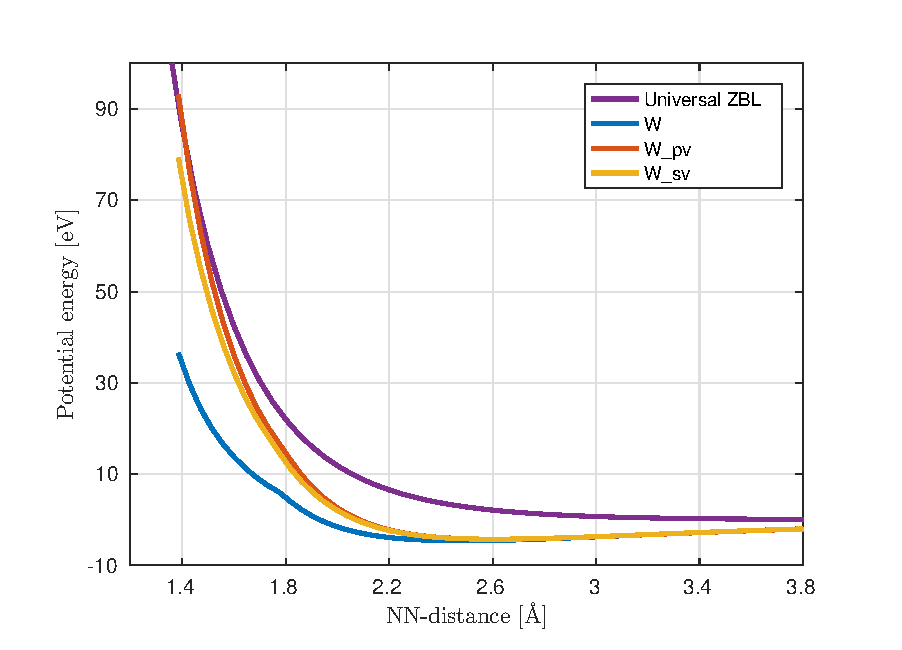
\includegraphics[scale=0.82]{img/pot-comp-compr2.eps}
  \caption{Comparing the two potential models by varying the lattice constant.}
  \label{fig:compr-comp}
\end{figure}

\begin{thebibliography}{100}
  % \addcontentsline{toc}{chapter}{\bibname}
\bibitem{Pseudopot} \url{https://commons.wikimedia.org/wiki/File:Sketch_Pseudopotentials.png}
\end{thebibliography}

\end{document}